\documentclass[aspectratio=169,11pt]{beamer}
% =====================================================================
%  pds-beamer.tex — Estilo común de las transparencias.
%
%  Uso (desde teoría/Tx/transparencias/):
%     \documentclass[aspectratio=169,11pt]{beamer}
%     % =====================================================================
%  pds-beamer.tex — Estilo común de las transparencias.
%
%  Uso (desde teoría/Tx/transparencias/):
%     \documentclass[aspectratio=169,11pt]{beamer}
%     % =====================================================================
%  pds-beamer.tex — Estilo común de las transparencias.
%
%  Uso (desde teoría/Tx/transparencias/):
%     \documentclass[aspectratio=169,11pt]{beamer}
%     \input{../../comun/pds-beamer}
%     \title{...}  \subtitle{Tema x · ...}
%     \begin{document}
%       \portada
%       ...
%     \end{document}
%  Compilar con:  latexmk -xelatex  (o «make» desde teoría/)
% =====================================================================

\usetheme{Boadilla}
\usecolortheme{orchid}
\usefonttheme{professionalfonts}
\setbeamercovered{transparent}
\setbeamersize{text margin left=0.8cm, text margin right=0.8cm}
\setbeamertemplate{navigation symbols}{}
\setbeamertemplate{itemize item}[square]
\setbeamertemplate{itemize subitem}[circle]
\setbeamertemplate{itemize subsubitem}[triangle]
\setbeamertemplate{enumerate item}[square]
\setbeamertemplate{enumerate subitem}[circle]
\setbeamertemplate{caption}{\raggedright\insertcaption\par}

\input{../../comun/pds-comun.tex}

% Tipografía: Fira Sans + Fira Math (legibles en proyector)
\usepackage{fontspec}
\usepackage{unicode-math}
% Se cargan por nombre de fichero para que funcionen con cualquier
% instalación de TeX Live (o MiKTeX) sin instalar fuentes en el sistema.
\setmainfont{FiraSans}[Extension=.otf, UprightFont=*-Regular, BoldFont=*-SemiBold,
  ItalicFont=*-Italic, BoldItalicFont=*-SemiBoldItalic]
\setsansfont{FiraSans}[Extension=.otf, UprightFont=*-Regular, BoldFont=*-SemiBold,
  ItalicFont=*-Italic, BoldItalicFont=*-SemiBoldItalic]
\setmonofont{FiraMono}[Extension=.otf, UprightFont=*-Regular, BoldFont=*-Medium, AutoFakeSlant=0.15, Scale=0.92]
\setmathfont{FiraMath-Regular.otf}
\setmathfont{latinmodern-math.otf}[range={"229B,"22EE,"22F1}]

% Colores del tema ajustados a la paleta común (más contraste)
\setbeamercolor{structure}{fg=pdsazul}
\setbeamercolor{alerted text}{fg=pdsrojo}
\setbeamercolor{example text}{fg=pdsverde}
\setbeamercolor{block title}{bg=pdsazul, fg=white}
\setbeamercolor{block body}{bg=pdsfondo}
\setbeamercolor{block title alerted}{bg=pdsrojo, fg=white}
\setbeamercolor{block body alerted}{bg=pdsrojo!6}
\setbeamercolor{block title example}{bg=pdsverde, fg=white}
\setbeamercolor{block body example}{bg=pdsverde!6}
\setbeamercolor{frametitle}{fg=pdsazul, bg=white}
\setbeamerfont{frametitle}{size=\large, series=\bfseries}
\setbeamerfont{block title}{size=\normalsize, series=\bfseries}
\setbeamertemplate{blocks}[rounded][shadow=false]

% Logo en la esquina superior derecha de cada transparencia
\pgfdeclareimage[height=0.8cm]{logo}{../../comun/ucm.png}
\addtobeamertemplate{frametitle}{}{%
  \begin{tikzpicture}[remember picture, overlay]
    \node[anchor=north east, inner sep=0pt] at ([xshift=-0.25cm, yshift=-0.2cm]current page.north east) {\pgfuseimage{logo}};
  \end{tikzpicture}}

% Datos de portada
\author[\autorescorto]{\autores}
\institute[UCM]{\footnotesize\departamento\\\universidad}
\date[\curso]{\footnotesize\grado\\\curso}

\newcommand{\portada}{%
  \begin{frame}[plain]
    \begin{center}
      
\includegraphics[height=1.9cm]{../../comun/ucm.png}
    \end{center}
    \vspace{-0.4cm}
    \titlepage
  \end{frame}}

% Índice al empezar cada sección
\AtBeginSection[]{%
  \begin{frame}{Contenido}
    \tableofcontents[currentsection, hideothersubsections]
  \end{frame}}

\renewcommand{\pdscodesize}{\scriptsize}

% Utilidades
% \herramienta{T1-convolucion-continua}: enlace a la página publicada de
% herramientas/html (se abre en el navegador, sin instalar nada).
% \herramientaservidor{server/....py}: app que necesita Python (bokeh serve).
\newcommand{\urlherramientas}{https://ucm-237.github.io/PdS/}
\newcommand{\herramienta}[1]{%
  \par\vfill\hfill{\scriptsize\color{pdsgris}\faIcon\ \href{\urlherramientas#1.html}{Herramienta interactiva: \texttt{#1}}}}
\newcommand{\herramientaservidor}[1]{%
  \par\vfill\hfill{\scriptsize\color{pdsgris}\faIcon\ Herramienta interactiva (con Python): \texttt{herramientas/#1}}}
\newcommand{\faIcon}{\textbf{▶}}
\newcommand{\gris}[1]{{\color{pdsgris}#1}}
\newcommand{\nota}[1]{\par\vspace{2pt}{\footnotesize\color{pdsgris}\textit{#1}}\par}
% Nota sobre una errata de versiones anteriores (solo con \ERRATAS)
\newcommand{\errata}[1]{\iferratas\nota{Errata de versiones anteriores: #1}\fi}
\newcommand{\apuntes}[1]{\nota{Más detalle en los apuntes, #1.}}

% Bloques con nombre en castellano
\newenvironment{definicion}[1][Definición]{\begin{block}{#1}}{\end{block}}
\newenvironment{importante}[1][Importante]{\begin{alertblock}{#1}}{\end{alertblock}}
\newenvironment{ejemplo}[1][Ejemplo]{\begin{exampleblock}{#1}}{\end{exampleblock}}

%     \title{...}  \subtitle{Tema x · ...}
%     \begin{document}
%       \portada
%       ...
%     \end{document}
%  Compilar con:  latexmk -xelatex  (o «make» desde teoría/)
% =====================================================================

\usetheme{Boadilla}
\usecolortheme{orchid}
\usefonttheme{professionalfonts}
\setbeamercovered{transparent}
\setbeamersize{text margin left=0.8cm, text margin right=0.8cm}
\setbeamertemplate{navigation symbols}{}
\setbeamertemplate{itemize item}[square]
\setbeamertemplate{itemize subitem}[circle]
\setbeamertemplate{itemize subsubitem}[triangle]
\setbeamertemplate{enumerate item}[square]
\setbeamertemplate{enumerate subitem}[circle]
\setbeamertemplate{caption}{\raggedright\insertcaption\par}

% =====================================================================
%  pds-comun.tex — Paquetes, colores y estilos de código comunes a
%  transparencias, apuntes y hojas de ejercicios. Compilar con XeLaTeX.
%  No cargar directamente: lo cargan pds-beamer.tex y pds-apuntes.tex.
% =====================================================================

\usepackage{polyglossia}
\setmainlanguage{spanish}
\usepackage{mathtools}
\usepackage{graphicx}
\usepackage{booktabs}
\usepackage{multirow}
\usepackage{array}
\usepackage{xcolor}
\usepackage{tikz}
\usetikzlibrary{positioning,arrows.meta,calc,shapes.geometric,decorations.pathreplacing}
\usepackage{listings}
\usepackage{siunitx}
\sisetup{output-decimal-marker={,}, group-separator={\,}, per-mode=symbol}

% Notas de erratas de versiones anteriores: no se imprimen salvo que se
% defina \ERRATAS antes de cargar el estilo (make ERRATAS=1)
\newif\iferratas
\ifdefined\ERRATAS \erratastrue \fi

% Ruta común (logo y figuras compartidas)
\providecommand{\rutacomun}{../../comun/}
\input{\rutacomun datos.tex}

% ---------------------------------------------------------------------
%  Paleta (la misma que usan las figuras generadas con Python,
%  ver comun/pds_estilo.py)
% ---------------------------------------------------------------------
\definecolor{pdsazul}{HTML}{2B3A8C}
\definecolor{pdsrojo}{HTML}{C0392B}
\definecolor{pdsverde}{HTML}{1E7B4F}
\definecolor{pdsnaranja}{HTML}{D9822B}
\definecolor{pdsgris}{HTML}{5A5A66}
\definecolor{pdsfondo}{HTML}{F3F4FA}
\definecolor{pdscodigo}{HTML}{F7F7F2}

% ---------------------------------------------------------------------
%  Diagramas de bloques (TikZ)
% ---------------------------------------------------------------------
\tikzset{
  bloque/.style={rectangle, rounded corners=2pt, draw=pdsazul!80, fill=pdsfondo,
                 very thick, minimum height=8mm, minimum width=14mm, align=center},
  sumador/.style={circle, draw=pdsazul!80, fill=pdsfondo, thick, inner sep=1.5pt},
  flecha/.style={-{Stealth[length=2.2mm]}, thick, pdsgris},
}

% ---------------------------------------------------------------------
%  Código: Python y Matlab en paralelo
% ---------------------------------------------------------------------
\newcommand{\pdscodesize}{\footnotesize}
\lstdefinestyle{pds}{
  basicstyle=\ttfamily\pdscodesize,
  keywordstyle=\color{pdsazul}\bfseries,
  commentstyle=\color{pdsverde}\itshape,
  stringstyle=\color{pdsrojo},
  numbers=none,
  backgroundcolor=\color{pdscodigo},
  frame=single, rulecolor=\color{pdsgris!40}, framerule=0.4pt,
  xleftmargin=2pt, xrightmargin=2pt, aboveskip=2pt, belowskip=2pt,
  columns=fullflexible, keepspaces=true,
  showstringspaces=false, breaklines=true, tabsize=4,
  upquote=true,
  % Con XeLaTeX, listings desordena los caracteres no ASCII junto a
  % dígitos («2π» sale «π2»): se sustituyen por su versión matemática.
  literate={π}{{$\pi$}}1 {δ}{{$\delta$}}1 {ω}{{$\omega$}}1 {Ω}{{$\Omega$}}1
           {≈}{{$\approx$}}1 {µ}{{$\mu$}}1 {·}{{$\cdot$}}1 {α}{{$\alpha$}}1
           {á}{{á}}1 {é}{{é}}1 {í}{{í}}1 {ó}{{ó}}1 {ú}{{ú}}1 {ñ}{{ñ}}1 {¿}{{¿}}1,
}
\lstdefinestyle{python}{style=pds, language=Python,
  morekeywords={as,True,False,None}}
\lstdefinestyle{matlab}{style=pds, language=Matlab,
  morekeywords={function,end,true,false}}

% \codigo{<ruta sin extensión>} muestra el mismo ejemplo en Python
% y en Matlab, uno al lado del otro. Los ficheros viven en
% ../codigo/python/<nombre>.py y ../codigo/matlab/<nombre>.m y se
% ejecutan en las pruebas (make prueba-codigo).
\newcommand{\rutacodigo}{../codigo/}
\newcommand{\codigoetiqueta}[1]{{\sffamily\scriptsize\bfseries\color{pdsgris}#1}}
\newcommand{\codigo}[2][]{%
  \par\noindent
  \begin{minipage}[t]{0.495\linewidth}
    \codigoetiqueta{Python}\par\vspace{1pt}
    \lstinputlisting[style=python,#1]{\rutacodigo python/#2.py}
  \end{minipage}\hfill
  \begin{minipage}[t]{0.495\linewidth}
    \codigoetiqueta{Matlab}\par\vspace{1pt}
    \lstinputlisting[style=matlab,#1]{\rutacodigo matlab/#2.m}
  \end{minipage}\par}

\input{\rutacomun notacion.tex}


% Tipografía: Fira Sans + Fira Math (legibles en proyector)
\usepackage{fontspec}
\usepackage{unicode-math}
% Se cargan por nombre de fichero para que funcionen con cualquier
% instalación de TeX Live (o MiKTeX) sin instalar fuentes en el sistema.
\setmainfont{FiraSans}[Extension=.otf, UprightFont=*-Regular, BoldFont=*-SemiBold,
  ItalicFont=*-Italic, BoldItalicFont=*-SemiBoldItalic]
\setsansfont{FiraSans}[Extension=.otf, UprightFont=*-Regular, BoldFont=*-SemiBold,
  ItalicFont=*-Italic, BoldItalicFont=*-SemiBoldItalic]
\setmonofont{FiraMono}[Extension=.otf, UprightFont=*-Regular, BoldFont=*-Medium, AutoFakeSlant=0.15, Scale=0.92]
\setmathfont{FiraMath-Regular.otf}
\setmathfont{latinmodern-math.otf}[range={"229B,"22EE,"22F1}]

% Colores del tema ajustados a la paleta común (más contraste)
\setbeamercolor{structure}{fg=pdsazul}
\setbeamercolor{alerted text}{fg=pdsrojo}
\setbeamercolor{example text}{fg=pdsverde}
\setbeamercolor{block title}{bg=pdsazul, fg=white}
\setbeamercolor{block body}{bg=pdsfondo}
\setbeamercolor{block title alerted}{bg=pdsrojo, fg=white}
\setbeamercolor{block body alerted}{bg=pdsrojo!6}
\setbeamercolor{block title example}{bg=pdsverde, fg=white}
\setbeamercolor{block body example}{bg=pdsverde!6}
\setbeamercolor{frametitle}{fg=pdsazul, bg=white}
\setbeamerfont{frametitle}{size=\large, series=\bfseries}
\setbeamerfont{block title}{size=\normalsize, series=\bfseries}
\setbeamertemplate{blocks}[rounded][shadow=false]

% Logo en la esquina superior derecha de cada transparencia
\pgfdeclareimage[height=0.8cm]{logo}{../../comun/ucm.png}
\addtobeamertemplate{frametitle}{}{%
  \begin{tikzpicture}[remember picture, overlay]
    \node[anchor=north east, inner sep=0pt] at ([xshift=-0.25cm, yshift=-0.2cm]current page.north east) {\pgfuseimage{logo}};
  \end{tikzpicture}}

% Datos de portada
\author[\autorescorto]{\autores}
\institute[UCM]{\footnotesize\departamento\\\universidad}
\date[\curso]{\footnotesize\grado\\\curso}

\newcommand{\portada}{%
  \begin{frame}[plain]
    \begin{center}
      
\includegraphics[height=1.9cm]{../../comun/ucm.png}
    \end{center}
    \vspace{-0.4cm}
    \titlepage
  \end{frame}}

% Índice al empezar cada sección
\AtBeginSection[]{%
  \begin{frame}{Contenido}
    \tableofcontents[currentsection, hideothersubsections]
  \end{frame}}

\renewcommand{\pdscodesize}{\scriptsize}

% Utilidades
% \herramienta{T1-convolucion-continua}: enlace a la página publicada de
% herramientas/html (se abre en el navegador, sin instalar nada).
% \herramientaservidor{server/....py}: app que necesita Python (bokeh serve).
\newcommand{\urlherramientas}{https://ucm-237.github.io/PdS/}
\newcommand{\herramienta}[1]{%
  \par\vfill\hfill{\scriptsize\color{pdsgris}\faIcon\ \href{\urlherramientas#1.html}{Herramienta interactiva: \texttt{#1}}}}
\newcommand{\herramientaservidor}[1]{%
  \par\vfill\hfill{\scriptsize\color{pdsgris}\faIcon\ Herramienta interactiva (con Python): \texttt{herramientas/#1}}}
\newcommand{\faIcon}{\textbf{▶}}
\newcommand{\gris}[1]{{\color{pdsgris}#1}}
\newcommand{\nota}[1]{\par\vspace{2pt}{\footnotesize\color{pdsgris}\textit{#1}}\par}
% Nota sobre una errata de versiones anteriores (solo con \ERRATAS)
\newcommand{\errata}[1]{\iferratas\nota{Errata de versiones anteriores: #1}\fi}
\newcommand{\apuntes}[1]{\nota{Más detalle en los apuntes, #1.}}

% Bloques con nombre en castellano
\newenvironment{definicion}[1][Definición]{\begin{block}{#1}}{\end{block}}
\newenvironment{importante}[1][Importante]{\begin{alertblock}{#1}}{\end{alertblock}}
\newenvironment{ejemplo}[1][Ejemplo]{\begin{exampleblock}{#1}}{\end{exampleblock}}

%     \title{...}  \subtitle{Tema x · ...}
%     \begin{document}
%       \portada
%       ...
%     \end{document}
%  Compilar con:  latexmk -xelatex  (o «make» desde teoría/)
% =====================================================================

\usetheme{Boadilla}
\usecolortheme{orchid}
\usefonttheme{professionalfonts}
\setbeamercovered{transparent}
\setbeamersize{text margin left=0.8cm, text margin right=0.8cm}
\setbeamertemplate{navigation symbols}{}
\setbeamertemplate{itemize item}[square]
\setbeamertemplate{itemize subitem}[circle]
\setbeamertemplate{itemize subsubitem}[triangle]
\setbeamertemplate{enumerate item}[square]
\setbeamertemplate{enumerate subitem}[circle]
\setbeamertemplate{caption}{\raggedright\insertcaption\par}

% =====================================================================
%  pds-comun.tex — Paquetes, colores y estilos de código comunes a
%  transparencias, apuntes y hojas de ejercicios. Compilar con XeLaTeX.
%  No cargar directamente: lo cargan pds-beamer.tex y pds-apuntes.tex.
% =====================================================================

\usepackage{polyglossia}
\setmainlanguage{spanish}
\usepackage{mathtools}
\usepackage{graphicx}
\usepackage{booktabs}
\usepackage{multirow}
\usepackage{array}
\usepackage{xcolor}
\usepackage{tikz}
\usetikzlibrary{positioning,arrows.meta,calc,shapes.geometric,decorations.pathreplacing}
\usepackage{listings}
\usepackage{siunitx}
\sisetup{output-decimal-marker={,}, group-separator={\,}, per-mode=symbol}

% Notas de erratas de versiones anteriores: no se imprimen salvo que se
% defina \ERRATAS antes de cargar el estilo (make ERRATAS=1)
\newif\iferratas
\ifdefined\ERRATAS \erratastrue \fi

% Ruta común (logo y figuras compartidas)
\providecommand{\rutacomun}{../../comun/}
\input{\rutacomun datos.tex}

% ---------------------------------------------------------------------
%  Paleta (la misma que usan las figuras generadas con Python,
%  ver comun/pds_estilo.py)
% ---------------------------------------------------------------------
\definecolor{pdsazul}{HTML}{2B3A8C}
\definecolor{pdsrojo}{HTML}{C0392B}
\definecolor{pdsverde}{HTML}{1E7B4F}
\definecolor{pdsnaranja}{HTML}{D9822B}
\definecolor{pdsgris}{HTML}{5A5A66}
\definecolor{pdsfondo}{HTML}{F3F4FA}
\definecolor{pdscodigo}{HTML}{F7F7F2}

% ---------------------------------------------------------------------
%  Diagramas de bloques (TikZ)
% ---------------------------------------------------------------------
\tikzset{
  bloque/.style={rectangle, rounded corners=2pt, draw=pdsazul!80, fill=pdsfondo,
                 very thick, minimum height=8mm, minimum width=14mm, align=center},
  sumador/.style={circle, draw=pdsazul!80, fill=pdsfondo, thick, inner sep=1.5pt},
  flecha/.style={-{Stealth[length=2.2mm]}, thick, pdsgris},
}

% ---------------------------------------------------------------------
%  Código: Python y Matlab en paralelo
% ---------------------------------------------------------------------
\newcommand{\pdscodesize}{\footnotesize}
\lstdefinestyle{pds}{
  basicstyle=\ttfamily\pdscodesize,
  keywordstyle=\color{pdsazul}\bfseries,
  commentstyle=\color{pdsverde}\itshape,
  stringstyle=\color{pdsrojo},
  numbers=none,
  backgroundcolor=\color{pdscodigo},
  frame=single, rulecolor=\color{pdsgris!40}, framerule=0.4pt,
  xleftmargin=2pt, xrightmargin=2pt, aboveskip=2pt, belowskip=2pt,
  columns=fullflexible, keepspaces=true,
  showstringspaces=false, breaklines=true, tabsize=4,
  upquote=true,
  % Con XeLaTeX, listings desordena los caracteres no ASCII junto a
  % dígitos («2π» sale «π2»): se sustituyen por su versión matemática.
  literate={π}{{$\pi$}}1 {δ}{{$\delta$}}1 {ω}{{$\omega$}}1 {Ω}{{$\Omega$}}1
           {≈}{{$\approx$}}1 {µ}{{$\mu$}}1 {·}{{$\cdot$}}1 {α}{{$\alpha$}}1
           {á}{{á}}1 {é}{{é}}1 {í}{{í}}1 {ó}{{ó}}1 {ú}{{ú}}1 {ñ}{{ñ}}1 {¿}{{¿}}1,
}
\lstdefinestyle{python}{style=pds, language=Python,
  morekeywords={as,True,False,None}}
\lstdefinestyle{matlab}{style=pds, language=Matlab,
  morekeywords={function,end,true,false}}

% \codigo{<ruta sin extensión>} muestra el mismo ejemplo en Python
% y en Matlab, uno al lado del otro. Los ficheros viven en
% ../codigo/python/<nombre>.py y ../codigo/matlab/<nombre>.m y se
% ejecutan en las pruebas (make prueba-codigo).
\newcommand{\rutacodigo}{../codigo/}
\newcommand{\codigoetiqueta}[1]{{\sffamily\scriptsize\bfseries\color{pdsgris}#1}}
\newcommand{\codigo}[2][]{%
  \par\noindent
  \begin{minipage}[t]{0.495\linewidth}
    \codigoetiqueta{Python}\par\vspace{1pt}
    \lstinputlisting[style=python,#1]{\rutacodigo python/#2.py}
  \end{minipage}\hfill
  \begin{minipage}[t]{0.495\linewidth}
    \codigoetiqueta{Matlab}\par\vspace{1pt}
    \lstinputlisting[style=matlab,#1]{\rutacodigo matlab/#2.m}
  \end{minipage}\par}

\input{\rutacomun notacion.tex}


% Tipografía: Fira Sans + Fira Math (legibles en proyector)
\usepackage{fontspec}
\usepackage{unicode-math}
% Se cargan por nombre de fichero para que funcionen con cualquier
% instalación de TeX Live (o MiKTeX) sin instalar fuentes en el sistema.
\setmainfont{FiraSans}[Extension=.otf, UprightFont=*-Regular, BoldFont=*-SemiBold,
  ItalicFont=*-Italic, BoldItalicFont=*-SemiBoldItalic]
\setsansfont{FiraSans}[Extension=.otf, UprightFont=*-Regular, BoldFont=*-SemiBold,
  ItalicFont=*-Italic, BoldItalicFont=*-SemiBoldItalic]
\setmonofont{FiraMono}[Extension=.otf, UprightFont=*-Regular, BoldFont=*-Medium, AutoFakeSlant=0.15, Scale=0.92]
\setmathfont{FiraMath-Regular.otf}
\setmathfont{latinmodern-math.otf}[range={"229B,"22EE,"22F1}]

% Colores del tema ajustados a la paleta común (más contraste)
\setbeamercolor{structure}{fg=pdsazul}
\setbeamercolor{alerted text}{fg=pdsrojo}
\setbeamercolor{example text}{fg=pdsverde}
\setbeamercolor{block title}{bg=pdsazul, fg=white}
\setbeamercolor{block body}{bg=pdsfondo}
\setbeamercolor{block title alerted}{bg=pdsrojo, fg=white}
\setbeamercolor{block body alerted}{bg=pdsrojo!6}
\setbeamercolor{block title example}{bg=pdsverde, fg=white}
\setbeamercolor{block body example}{bg=pdsverde!6}
\setbeamercolor{frametitle}{fg=pdsazul, bg=white}
\setbeamerfont{frametitle}{size=\large, series=\bfseries}
\setbeamerfont{block title}{size=\normalsize, series=\bfseries}
\setbeamertemplate{blocks}[rounded][shadow=false]

% Logo en la esquina superior derecha de cada transparencia
\pgfdeclareimage[height=0.8cm]{logo}{../../comun/ucm.png}
\addtobeamertemplate{frametitle}{}{%
  \begin{tikzpicture}[remember picture, overlay]
    \node[anchor=north east, inner sep=0pt] at ([xshift=-0.25cm, yshift=-0.2cm]current page.north east) {\pgfuseimage{logo}};
  \end{tikzpicture}}

% Datos de portada
\author[\autorescorto]{\autores}
\institute[UCM]{\footnotesize\departamento\\\universidad}
\date[\curso]{\footnotesize\grado\\\curso}

\newcommand{\portada}{%
  \begin{frame}[plain]
    \begin{center}
      
\includegraphics[height=1.9cm]{../../comun/ucm.png}
    \end{center}
    \vspace{-0.4cm}
    \titlepage
  \end{frame}}

% Índice al empezar cada sección
\AtBeginSection[]{%
  \begin{frame}{Contenido}
    \tableofcontents[currentsection, hideothersubsections]
  \end{frame}}

\renewcommand{\pdscodesize}{\scriptsize}

% Utilidades
% \herramienta{T1-convolucion-continua}: enlace a la página publicada de
% herramientas/html (se abre en el navegador, sin instalar nada).
% \herramientaservidor{server/....py}: app que necesita Python (bokeh serve).
\newcommand{\urlherramientas}{https://ucm-237.github.io/PdS/}
\newcommand{\herramienta}[1]{%
  \par\vfill\hfill{\scriptsize\color{pdsgris}\faIcon\ \href{\urlherramientas#1.html}{Herramienta interactiva: \texttt{#1}}}}
\newcommand{\herramientaservidor}[1]{%
  \par\vfill\hfill{\scriptsize\color{pdsgris}\faIcon\ Herramienta interactiva (con Python): \texttt{herramientas/#1}}}
\newcommand{\faIcon}{\textbf{▶}}
\newcommand{\gris}[1]{{\color{pdsgris}#1}}
\newcommand{\nota}[1]{\par\vspace{2pt}{\footnotesize\color{pdsgris}\textit{#1}}\par}
% Nota sobre una errata de versiones anteriores (solo con \ERRATAS)
\newcommand{\errata}[1]{\iferratas\nota{Errata de versiones anteriores: #1}\fi}
\newcommand{\apuntes}[1]{\nota{Más detalle en los apuntes, #1.}}

% Bloques con nombre en castellano
\newenvironment{definicion}[1][Definición]{\begin{block}{#1}}{\end{block}}
\newenvironment{importante}[1][Importante]{\begin{alertblock}{#1}}{\end{alertblock}}
\newenvironment{ejemplo}[1][Ejemplo]{\begin{exampleblock}{#1}}{\end{exampleblock}}

\graphicspath{{../figuras/}}

\title[T6 · Análisis espectral]{Señales aleatorias}
\subtitle{Tema 6 · Parte 4: análisis espectral y sistemas LTI}

\begin{document}
\portada

% =====================================================================
\section{Densidad espectral de potencia}

\begin{frame}{El espectro de una señal aleatoria}
  \small
  \begin{itemize}
    \item Una realización de una señal estacionaria no se apaga: tiene energía infinita y su DTFT no existe en sentido ordinario. Además, cada realización tendría un espectro distinto.
    \item Lo que sí está bien definido es su \alert{potencia} media:
    \[
      P_x=E\Big\{\lim_{N\to\infty}\frac1{2N+1}\sum_{n=-N}^Nx^2[n]\Big\}=E\{x^2[n]\}=\phi_{xx}[0]\quad\text{(ESA)}.
    \]
    \item La autocorrelación es una «potencia generalizada» que depende de la separación $l$. Su transformada dice cómo se reparte la potencia en frecuencia.
  \end{itemize}
  \begin{definicion}[Densidad espectral de potencia (DEP)]
    \[
      \Phi_{xx}(\e^{j\Omega})=\sum_{l=-\infty}^{\infty}\phi_{xx}[l]\,\e^{-j\Omega l},\qquad
      \phi_{xx}[l]=\frac1{2\pi}\int_{-\pi}^{\pi}\Phi_{xx}(\e^{j\Omega})\,\e^{j\Omega l}\dd\Omega .
    \]
  \end{definicion}
  \nota{Es el teorema de Wiener-Khinchin. En continuo: $\Phi_{xx}(j\omega)=\int\phi_{xx}(\tau)\e^{-j\omega\tau}\dd\tau$.}
\end{frame}

\begin{frame}{Propiedades}
  \small
  \begin{itemize}
    \item \alert{Potencia}: con $l=0$,
    \[
      P_x=\phi_{xx}[0]=\frac1{2\pi}\int_{-\pi}^{\pi}\Phi_{xx}(\e^{j\Omega})\dd\Omega .
    \]
    La potencia en una banda $[\Omega_1,\Omega_2]$ es $\frac1{2\pi}\int$ sobre $\pm[\Omega_1,\Omega_2]$: por eso es una \emph{densidad}.
    \item $\Phi_{xx}$ es \alert{real} (porque $\phi_{xx}$ es par), \alert{par} si $x$ es real, y \alert{no negativa}.
    \item Interpretación: $\Phi_{xx}(\e^{j\Omega})=\lim_{N\to\infty}\frac1{N}E\big\{\abs{X_N(\e^{j\Omega})}^2\big\}$, con $X_N$ la DTFT de $N$ muestras: el módulo al cuadrado del espectro, promediado.
    \item En continuo: $P_x=\frac1{2\pi}\int\Phi_{xx}(j\omega)\dd\omega=\int\Phi_{xx}(j2\pi f)\dd f$, en W/Hz si $x$ está en voltios sobre 1\,$\Omega$.
  \end{itemize}
  \nota{Las transparencias antiguas usaban $\omega$ también para la frecuencia discreta; aquí, como en todo el curso, $\Omega$.}
\end{frame}

\begin{frame}{Ejemplos}
  \begin{columns}[c]
    \begin{column}{0.47\textwidth}
      \footnotesize
      \begin{itemize}
        \item \alert{Ruido blanco}: $\phi_{xx}[l]=\sigma^2\delta[l]$ $\Rightarrow$ $\Phi_{xx}=\sigma^2$, plana.
        \item \alert{AR(1)}: $\phi_{xx}[l]=\frac{\sigma_w^2a^{\abs l}}{1-a^2}$ $\Rightarrow$
        \[
          \Phi_{xx}=\frac{\sigma_w^2}{\abs{1-a\e^{-j\Omega}}^2}=\frac{\sigma_w^2}{1-2a\cos\Omega+a^2}.
        \]
        Paso bajo si $a>0$, paso alto si $a<0$.
        \item \alert{Constante}: $\phi_{xx}[l]=\mu^2$ $\Rightarrow$ $\Phi_{xx}=2\pi\mu^2\delta(\Omega)$ en $[-\pi,\pi]$.
        \item \alert{Sinusoide de fase aleatoria}: $\frac{A^2}2\cos\Omega_0l$ $\Rightarrow$ $\frac{\pi A^2}2[\delta(\Omega-\Omega_0)+\delta(\Omega+\Omega_0)]$.
      \end{itemize}
    \end{column}
    \begin{column}{0.51\textwidth}
      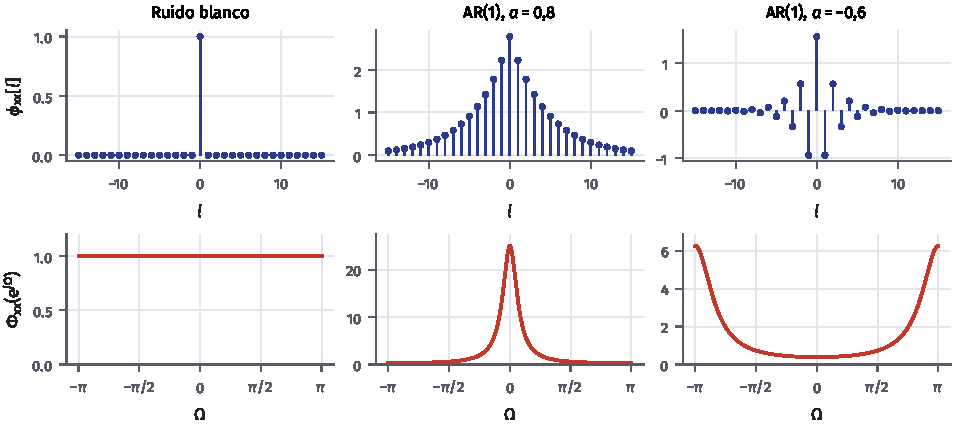
\includegraphics[width=\linewidth]{dep_ejemplos}
    \end{column}
  \end{columns}
  \nota{Errata antigua: la DEP de la constante se escribía $\mu^2\delta(\omega)$, sin el factor $2\pi$.}
\end{frame}

\begin{frame}{Clasificación y ruido blanco continuo}
  \small
  \begin{itemize}
    \item Según la forma de la DEP: \alert{blanca} (plana), \alert{de banda ancha}, \alert{de banda estrecha}, \alert{paso bajo}, \alert{paso banda}. «Coloreada» es cualquiera que no sea blanca.
    \item Una señal con DEP no nula en todas las frecuencias tiene muestras correladas a corta distancia: la anchura de $\phi_{xx}$ es inversa al ancho de banda.
  \end{itemize}
  \begin{importante}[Ruido blanco continuo]
    $\phi_{xx}(\tau)=\frac{N_0}2\delta(\tau)$ y $\Phi_{xx}=\frac{N_0}2$: tendría potencia $\phi_{xx}(0)=\infty$, así que no existe físicamente. Es un modelo para ruido cuya DEP es plana en toda la banda que interesa, por ejemplo el ruido térmico de una resistencia ($N_0/2=2kTR$\,V$^2$/Hz). Tras un paso bajo ideal de ancho $B$\,Hz, la potencia es $N_0B$.
  \end{importante}
  \nota{Al muestrear a $f_s=2B$ ruido blanco limitado a $B$\,Hz se obtiene ruido blanco discreto de varianza $N_0B$.}
\end{frame}

\begin{frame}{Densidad espectral cruzada}
  \small
  \[
    \Phi_{xy}(\e^{j\Omega})=\sum_{l=-\infty}^{\infty}\phi_{xy}[l]\,\e^{-j\Omega l}
  \]
  \begin{itemize}
    \item En general es \alert{compleja}: $\phi_{xy}$ no es par. Como $\phi_{yx}[l]=\phi_{xy}[-l]$, $\Phi_{yx}=\Phi_{xy}^*$ para señales reales.
    \item Su módulo dice en qué frecuencias $x$ e $y$ tienen potencia común; su fase, el desfase entre ellas.
    \item \alert{Coherencia}: $C_{xy}=\dfrac{\abs{\Phi_{xy}}^2}{\Phi_{xx}\Phi_{yy}}\in[0,1]$; vale 1 en las frecuencias donde $y$ es una versión filtrada de $x$ sin ruido.
  \end{itemize}
\end{frame}

% =====================================================================
\section{Respuesta de un sistema LTI}

\begin{frame}{Señal aleatoria a través de un sistema LTI}
  \small
  $y[n]=\sum_kh[k]\,x[n-k]$, con $h$ real y estable y $x$ ESA. La salida también es ESA y:
  \begin{itemize}
    \item \alert{Media}: $\mu_y=E\{\sum_kh[k]x[n-k]\}=\mu_x\sum_kh[k]=H(\e^{j0})\,\mu_x$.
    \item \alert{Correlación cruzada}:
    \(
      \phi_{yx}[l]=E\{y[n+l]x[n]\}=\sum_kh[k]\,\phi_{xx}[l-k]=(h\conv\phi_{xx})[l]
    \)
    \item \alert{Autocorrelación}:
    \(
      \phi_{yy}[l]=\sum_k\sum_rh[k]h[r]\,\phi_{xx}[l-k+r]=(h\conv\tilde h\conv\phi_{xx})[l],\quad\tilde h[n]=h[-n].
    \)
  \end{itemize}
  \begin{importante}[En frecuencia]
    \[
      \Phi_{yx}(\e^{j\Omega})=H(\e^{j\Omega})\,\Phi_{xx}(\e^{j\Omega}),\qquad
      \Phi_{yy}(\e^{j\Omega})=\abs{H(\e^{j\Omega})}^2\,\Phi_{xx}(\e^{j\Omega}).
    \]
  \end{importante}
  \nota{Las convoluciones se convierten en productos y $H(\e^{-j\Omega})=H^*(\e^{j\Omega})$. Potencia de salida: $\frac1{2\pi}\int\abs H^2\Phi_{xx}\dd\Omega$; con entrada blanca, $\sigma_x^2\sum_kh^2[k]$.}
\end{frame}

\begin{frame}{Ruido coloreado}
  \begin{center}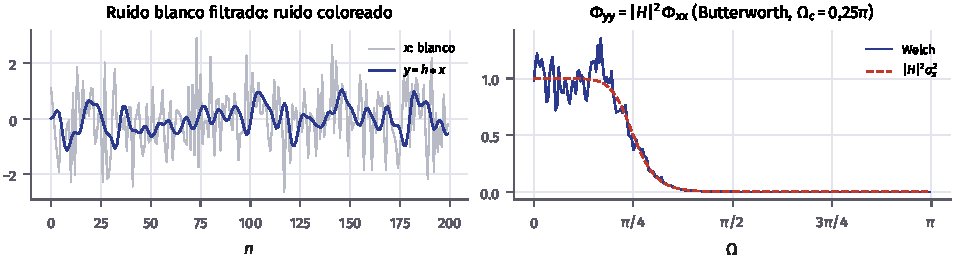
\includegraphics[width=0.95\linewidth]{filtrado_ruido}\end{center}
  \small
  \begin{itemize}
    \item Filtrar ruido blanco da ruido con la DEP que se quiera: $\Phi_{yy}=\sigma_x^2\abs H^2$. Así se simulan perturbaciones realistas, y el AR(1) es ruido blanco tras $1/(1-az^{-1})$.
    \item Al revés, un filtro \alert{blanqueador} $1/H$ convierte ruido coloreado en blanco.
    \item El filtro solo cambia la potencia de cada frecuencia; no puede crear frecuencias que no estaban.
  \end{itemize}
\end{frame}

\begin{frame}{Identificación de sistemas}
  \begin{columns}[c]
    \begin{column}{0.46\textwidth}
      \footnotesize
      \begin{itemize}
        \item Se excita un sistema desconocido con ruido de DEP conocida y se miden entrada y salida:
        \[
          \hat H(\e^{j\Omega})=\frac{\Phi_{yx}(\e^{j\Omega})}{\Phi_{xx}(\e^{j\Omega})}
        \]
        da módulo \alert{y fase}.
        \item $\abs H^2=\Phi_{yy}/\Phi_{xx}$ da solo el módulo, y el ruido de medida a la salida lo sesga; en $\Phi_{yx}$ ese ruido, incorrelado con $x$, desaparece al promediar.
        \item Con entrada blanca, $\phi_{yx}[l]=\sigma_x^2\,h[l]$: la correlación cruzada \emph{es} la respuesta al impulso.
      \end{itemize}
    \end{column}
    \begin{column}{0.52\textwidth}
      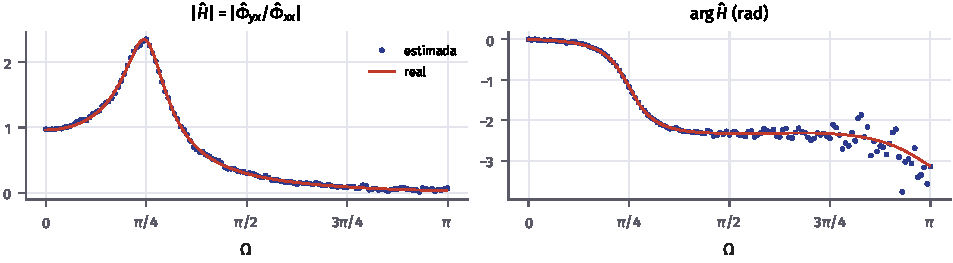
\includegraphics[width=\linewidth]{identificacion}
      \nota{$H(z)=\frac{0{,}2+0{,}3z^{-1}}{1-1{,}2z^{-1}+0{,}72z^{-2}}$, ruido de medida de $\sigma=0{,}3$. Donde $\abs H$ es pequeño, la fase se estima peor.}
    \end{column}
  \end{columns}
\end{frame}

\begin{frame}{En código: identificar un sistema}
  \codigo{identificacion}
  \nota{\texttt{scipy.signal.csd(x, y)} calcula $X^*Y$, que es $\Phi_{yx}$ con nuestro convenio.}
\end{frame}

% =====================================================================
\section{Estimación de la DEP}

\begin{frame}{Periodograma}
  \footnotesize
  \begin{itemize}
    \item Con $N$ muestras, lo inmediato es el \alert{periodograma}:
    \[
      I_N(\e^{j\Omega})=\frac1N\abs{\sum_{n=0}^{N-1}x[n]\,\e^{-j\Omega n}}^2,
    \]
    que es la DTFT de la autocorrelación estimada con el estimador sesgado. Se calcula con la FFT.
    \item Es asintóticamente insesgado (su media tiende a $\Phi_{xx}$), pero su varianza \alert{no disminuye} con $N$: es del orden de $\Phi_{xx}^2$. Más muestras dan más frecuencias, igual de ruidosas.
  \end{itemize}
  \begin{center}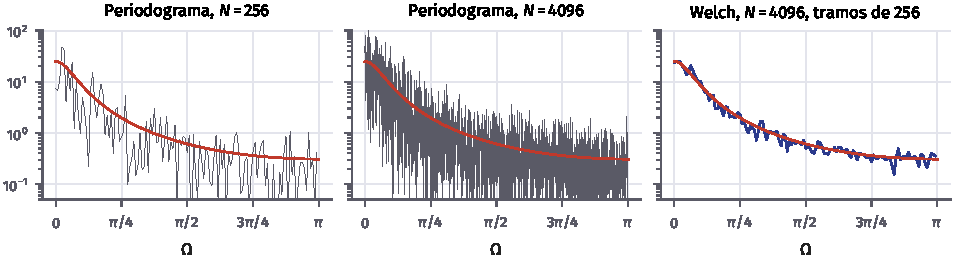
\includegraphics[width=0.78\linewidth]{periodograma}\end{center}
\end{frame}

\begin{frame}{Método de Welch}
  \small
  \begin{itemize}
    \item Se divide la señal en $K$ tramos de $L$ muestras (con solapamiento, típicamente del 50\,\%), se enventana cada uno, se calcula su periodograma y se \alert{promedian}.
    \item La varianza baja aproximadamente en un factor $K$ (algo menos con solapamiento); la resolución en frecuencia empeora a la de una ventana de $L$ muestras. Es el compromiso de la STFT del tema~5.
    \item Bartlett: lo mismo sin ventana ni solapamiento.
    \item Matlab: \texttt{pwelch}, \texttt{cpsd}, \texttt{tfestimate}, \texttt{mscohere}. Python: \texttt{scipy.signal.welch}, \texttt{csd}, \texttt{coherence}.
  \end{itemize}
  \begin{importante}[Escalas]
    Por defecto devuelven la DEP \emph{unilateral} (doble en $0<f<f_s/2$) y por unidad de frecuencia (Hz, o rad/muestra si no se da $f_s$). Con la opción bilateral y $f_s=1$ se obtiene $\Phi_{xx}(\e^{j2\pi f})$.
  \end{importante}
\end{frame}

\begin{frame}{En código: DEP de un AR(1) con Welch}
  \codigo{welch}
  \nota{Teórico, con $a=0{,}8$: $\Phi_{xx}(\e^{j0})=1/(1-a)^2=25$, $\Phi_{xx}(\e^{j\pi/2})=1/(1+a^2)=0{,}61$ y potencia $1/(1-a^2)=2{,}78$. El valor en 0 se estima peor porque la ventana ensancha el pico.}
\end{frame}

\begin{frame}{Aplicaciones}
  \begin{itemize}
    \item \alert{Medir el ruido} de un sistema y su relación señal a ruido por bandas.
    \item \alert{Detectar tonos} débiles en ruido: tras promediar, un tono destaca sobre un fondo cuya varianza se ha reducido.
    \item \alert{Identificar sistemas} y medir su respuesta en frecuencia en funcionamiento, sin desconectarlos.
    \item \alert{Filtro de Wiener}: para separar una señal $s$ de un ruido aditivo $v$ incorrelado, el filtro lineal óptimo es
    \[
      H(\e^{j\Omega})=\frac{\Phi_{ss}(\e^{j\Omega})}{\Phi_{ss}(\e^{j\Omega})+\Phi_{vv}(\e^{j\Omega})}:
    \]
    deja pasar las frecuencias donde domina la señal y atenúa donde domina el ruido.
  \end{itemize}
\end{frame}

% =====================================================================
\section*{Resumen}
\begin{frame}{Conceptos importantes}
  \begin{columns}[T]
    \begin{column}{0.5\textwidth}
      \begin{itemize}
        \item DEP: $\Phi_{xx}=\text{DTFT}\{\phi_{xx}\}$; real, par, $\ge0$.
        \item $P_x=\phi_{xx}[0]=\frac1{2\pi}\int\Phi_{xx}\dd\Omega$.
        \item Blanco: plana. AR(1): $\sigma_w^2/\abs{1-a\e^{-j\Omega}}^2$.
        \item DEP cruzada $\Phi_{xy}$, compleja; coherencia.
      \end{itemize}
    \end{column}
    \begin{column}{0.5\textwidth}
      \begin{itemize}
        \item LTI: $\mu_y=H(\e^{j0})\mu_x$, $\Phi_{yx}=H\Phi_{xx}$, $\Phi_{yy}=\abs H^2\Phi_{xx}$.
        \item Identificación: $\hat H=\Phi_{yx}/\Phi_{xx}$.
        \item Periodograma: varianza que no baja; Welch promedia tramos.
      \end{itemize}
    \end{column}
  \end{columns}
  \bigskip
  \gris{Apuntes del Tema 6, sección 4 · Hoja de ejercicios, ejercicios 15–18.}
\end{frame}

\end{document}
